 
\subsection{Recipes for engineering templates}
\label{ssec:recipes_technical}

\TBD It is not clear (2020-11-19) whether data from maintenance
templates need to be reduced by the pipeline. This section and the
recipes described therein serves as a placeholder and may be removed
later.

The CLC coronagraph was removed from the baseline coronagraphic modes before FDR however the coronagraph would be technically available during engineering. At this stage the DRL will not have the corresponding recipes to use the CLC. However, if the need arises during commissioning or after to make the CLC mode available, its DRL recipe can be easily adapted from the baseline RAVC/CVC coronagraph recipes as it is related in design and usage.

%------------------------------------------------------------------------------------------------------------------
\subsubsection{Pupil imaging}\label{rec:metis_pupil_imaging}
\label{sssec:pupil_imaging}

\TBD This recipe refers to pupil imaging using the science
detectors. Presumably it only contains the most basic reduction
steps. There may have to be separate recipes for the various
subsystems.

\begin{recipedef}
  Name                 & \hyperref[rec:metis_pupil_imaging]{\REC{metis_pupil_imaging}}                     \\
  Purpose:             & Apply basic reduction to pupil imaging data.  \\
  Requirements:        & --                                            \\
  Type:                & Maintenance                                   \\
  Templates:           & \TPL{METIS_pup_lm}                            \\
                       & \TPL{METIS_pup_n}                             \\
  Input data:          & \hyperref[dataitem:lm_pupil_raw]{\RAW{LM_PUPIL_RAW}} or \hyperref[dataitem:n_pupil_raw]{\RAW{N_PUPIL_RAW}} \\
  Matched keywords:    & Detector ID                                   \\
  Algorithm            & \TBD                                          \\
  Output data:         & \hyperref[dataitem:lm_pupil_reduced]{\PROD{LM_PUPIL_REDUCED}} or \hyperref[dataitem:n_pupil_reduced]{\PROD{N_PUPIL_REDUCED}} \\
  Expected accuracies: & None                                          \\
  QC1 parameters:      & None                                          \\
\end{recipedef}

\clearpage
%------------------------------------------------------------------------------------------------------------------
\subsubsection{Chopper Home Position recipe \REC{metis_img_chophome}}\label{ssec:metisimgchophome}
The recipe \hyperref[rec:metis_img_chophome]{\REC{metis_img_chophome}} aims to detect chopper mirror zero positions. Currently it is foreseen on daily basis to be carried out, but is for sure necessary after switching on the chopper (e.g. after instrument interventions) or induced by unforeseen events like earthquakes (cf. Section "Chopper Home Position" in  \cite{METIS-calibration_plan}).

The procedure consists of measuring the position of a point source from the \ac{WCU}, that has been centred on the \ac{WFS} pyramid (in the K-band), in the \CODE{IMG_LM} mode.
Then, taking the respective positional metrology values of the \ac{WFS}-FS and the chopper,
% TODO: What is the FS in WFS-FS?
the relative coordinates between the \ac{WFS} Pyramid focal plane, and the science focal planes is established.
%  (the latter in plural because we have already calibrated the relative astrometry between between IMG-LM and IMG-N/LMS).

\begin{figure}[ht]
  \centering
  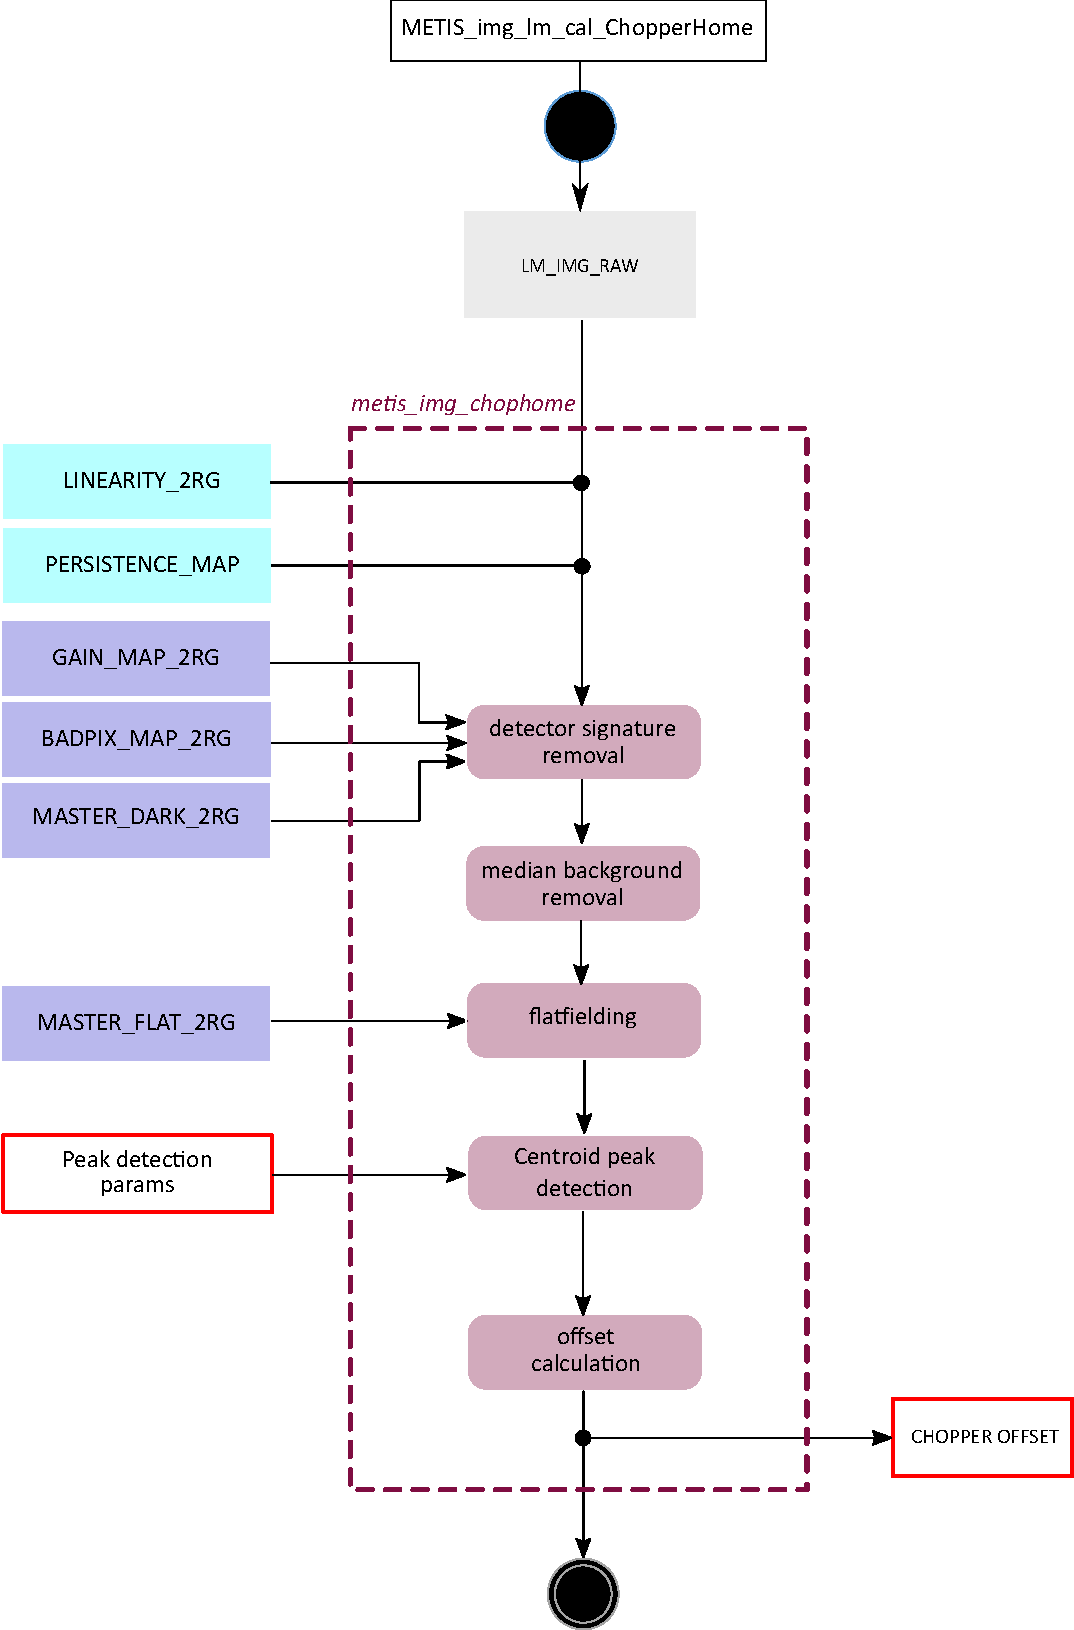
\includegraphics[width=0.5\textheight]{figures/metis_img_chophome_v0.83.pdf}
  \caption[Recipe: \REC{metis_img_chophome}]{\REC{metis_img_chophome} --
    Recipe workflow to detect the zero position of the chopper mirror.}
  \label{Fig:rec_chop_home}
\end{figure}

\begin{recipedef}\label{rec:metisimgchophome}\label{rec:metis_img_chophome}
Name:		& \hyperref[rec:metis_img_chophome]{\REC{metis_img_chophome}} \\
Purpose:	& Detection of the chopper mirror home position \\
Type:		& Calibration\\
Requirements: & TBD \\
Templates:      & \TPL{METIS_img_lm_cal_ChopperHome} \\
Input data:     & \hyperref[dataitem:lm_chopperhome_raw]{\RAW{LM_CHOPPERHOME_RAW}} \\
                & \hyperref[dataitem:persistence_map]{\EXTCALIB{PERSISTENCE_MAP}}  \\
                & \hyperref[dataitem:linearity_2rg]{\STATCALIB{LINEARITY_2RG}}  \\
                & \hyperref[dataitem:gain_map_2rg]{\PROD{GAIN_MAP_2RG}}  \\
                & \hyperref[dataitem:badpix_map_2rg]{\PROD{BADPIX_MAP_2RG}}  \\
                & \hyperref[dataitem:master_dark_2rg]{\PROD{MASTER_DARK_2RG}}  \\
                & \hyperref[dataitem:master_img_flat_lamp_lm]{\PROD{MASTER_IMG_FLAT_LAMP_LM}}  \\
Parameters: 	& TBD\\
Algorithm:      & remove detector signature\\
                & remove median background\\
                & apply flatfield\\
                & detect reference source from \ac{WCU} via centroid peak detection\\
                & Calculate mirror offset\\
Output data:	& Offset of the chopper mirror to be piped either into the \ac{ICS} for correction \\
                & or to be used in thee pipeline for astrometric correction\\
Expected accuracies: & 0.1mas accuracy of the centroid position (cf. \cite{METIS-calibration_plan})\\
QC1 parameters: & \QC{TBD}: TBD\\
\end{recipedef}
\clearpage

%------------------------------------------------------------------------------------------------------------------
% Moved to https://github.com/AstarVienna/METIS_DRLD/issues/101
% \subsubsection{Plate-scale calibration}
% \TODO{Plate-scale calibration}

%------------------------------------------------------------------------------------------------------------------
\subsubsection{Fringing correction}
\label{rec:metis_fringing_correction}

It is unclear for the time being how much of a problem will be with the METIS
detectors, and what the best strategy will be to tackle it. Therefore, the
method to use will be chosen based on AIT results (\REQ{METIS-9151}, for rationale and basic method description see Ch.~3.12 in the Calibration Plan \cite{METIS-calibration_plan}).

Whether a stand-alone recipe will be required, or if the fringe-map will become
part of another recipe, is part of that uncertainty. If needed, the design of
said recipe will be minimal work and is thus omitted in this document.

%------------------------------------------------------------------------------------------------------------------
\subsubsection{Slit loss determination recipes \REC{metis_lm/n\_adc\_slitloss}}\label{sssec:adc_slitlosses}
The recipes \hyperref[rec:metis_lm_adc_slitloss]{\REC{metis_lm_adc_slitloss}} (Fig.~\ref{Fig:rec_lm_adc_slitloss}) and \hyperref[rec:metis_n_adc_slitloss]{\REC{metis_n_adc_slitloss}} (Fig.~\ref{Fig:rec_n_adc_slitloss}) aims to determine the throughput as function of the object position along the across-slit direction. It is expected that the usage of the fixed positioned \ac{ADC} will introduce flux losses (cf. Section "Calibration of slit losses" in  \cite{METIS-calibration_plan}). For the determination, the point sources (i.e. mask of the \ac{WCU}) is placed on several positions (distance $\sim\frac{1}{10}\lambda/D$) across the slit (cf. Fig.~\ref{Fig:slitloss}), and measure the wavelength dependent flux changes with respect to the respective positions (see Section "Calibration of slit losses" in the Calibration Plan \cite{METIS-calibration_plan} for more details). Finally, parameters of a simple model (which is TBD) are determined to be able to correct for the flux losses. This recipe is to be carried out once in a while to update the static calibration database.
\begin{figure}[ht]
  \centering
  
\includegraphics[width=0.5\textheight]{figures/slitloss_det.pdf}
  \caption[slitloss determination]{Algorithm for the slit-loss determination in recipe \hyperref[rec:metis_lm_adc_slitloss]{\REC{metis_lm_adc_slitloss}} }
  \label{Fig:slitloss}
\end{figure}

\begin{figure}[ht]
  \centering
  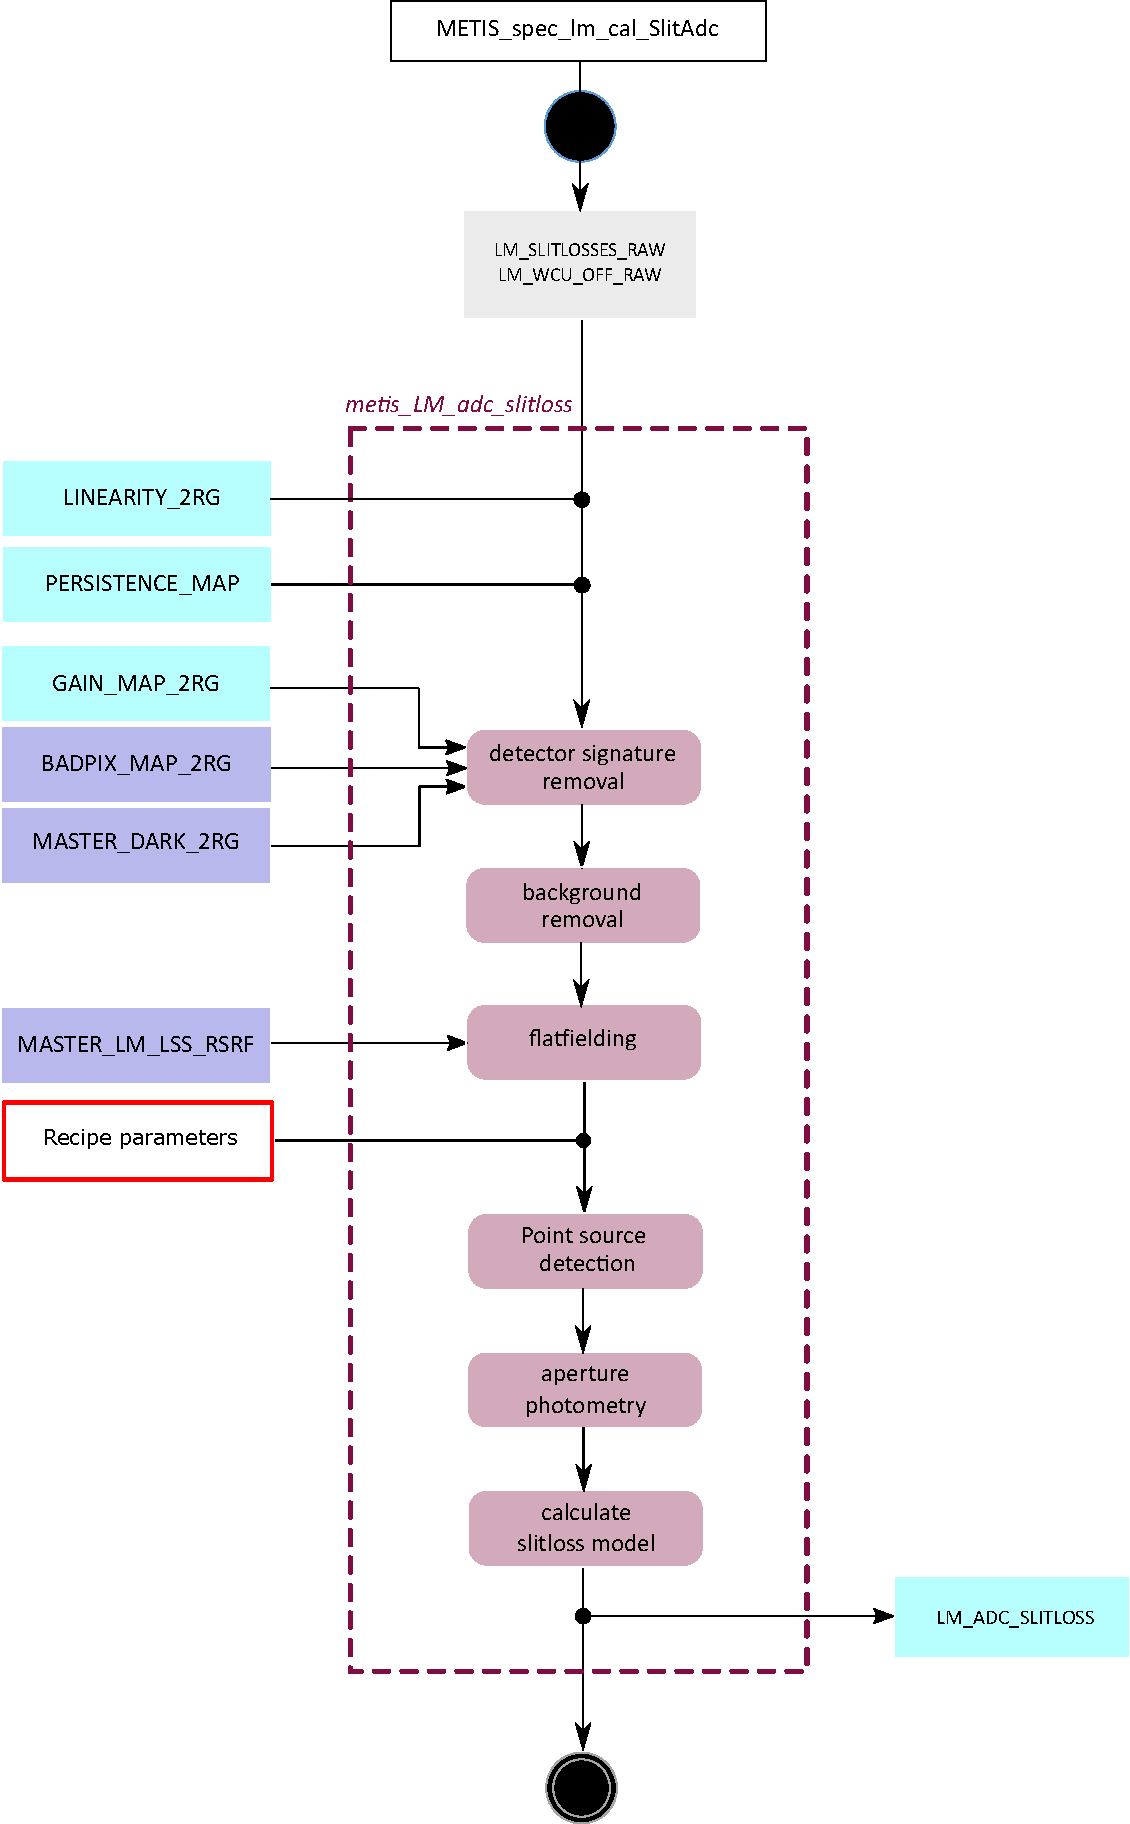
\includegraphics[width=0.5\textheight]{figures/metis_lm_lss_adc_slitloss_v0.83.pdf}
  \caption[Recipe: \REC{metis_lm_adc_slitloss}]{\REC{metis_lm_adc_slitloss} --
    Recipe workflow to determine the \ac{ADC} induced slit losses.}
  \label{Fig:rec_lm_adc_slitloss}
\end{figure}

\begin{recipedef}\label{rec:metislmadcmslitloss}\label{rec:metis_lm_adc_slitloss}
Name:		& \hyperref[rec:metis_lm_adc_slitloss]{\REC{metis_lm_adc_slitloss}} \\
Purpose:	& Determination of the \ac{ADC} induced slit losses \\
Type:		& Calibration\\
Requirements: &  METIS-6074, METIS-2757, METIS-9099, METIS-9150\\
Templates:           & \TPL{METIS_spec_lm_cal_SlitAdc} \\
Input data:     & \hyperref[dataitem:lm_slitlosses_raw]{\RAW{LM_SLITLOSSES_RAW}} \\
                & \hyperref[dataitem:lm_wcu_off_raw]{\RAW{LM_WCU_OFF_RAW}} \\
                & \hyperref[dataitem:persistence_map]{\EXTCALIB{PERSISTENCE_MAP}}  \\
                & \hyperref[dataitem:linearity_2rg]{\STATCALIB{LINEARITY_2RG}}  \\
                & \hyperref[dataitem:gain_map_2rg]{\PROD{GAIN_MAP_2RG}}  \\
                & \hyperref[dataitem:badpix_map_2rg]{\PROD{BADPIX_MAP_2RG}}  \\
                & \hyperref[dataitem:master_dark_2rg]{\PROD{MASTER_DARK_2RG}}  \\
                & \hyperref[dataitem:master_img_flat_lamp_lm]{\PROD{MASTER_IMG_FLAT_LAMP_LM}}  \\
Parameters: 	& exposure time, offset positions\\
Algorithm:      & remove detector signature\\
                & remove dark\\
                & apply flatfield\\
                & detect reference source from \ac{WCU} via centroid peak detection\\
                & apply aperture photometry\\
                & calculate (simple) slitloss model (details to be defined)\\
Output data:	& \hyperref[dataitem:lm_adc_slitloss]{\STATCALIB{LM_ADC_SLITLOSS}} (Slit loss model as function of the wavelength and object position across the slit \\
Expected accuracies: & 3\% (cf. \cite{METIS_calerrbudget})\\
%QC1 parameters: & \QC{TBD}: TBD\\
\end{recipedef}


\begin{figure}[ht]
  \centering
  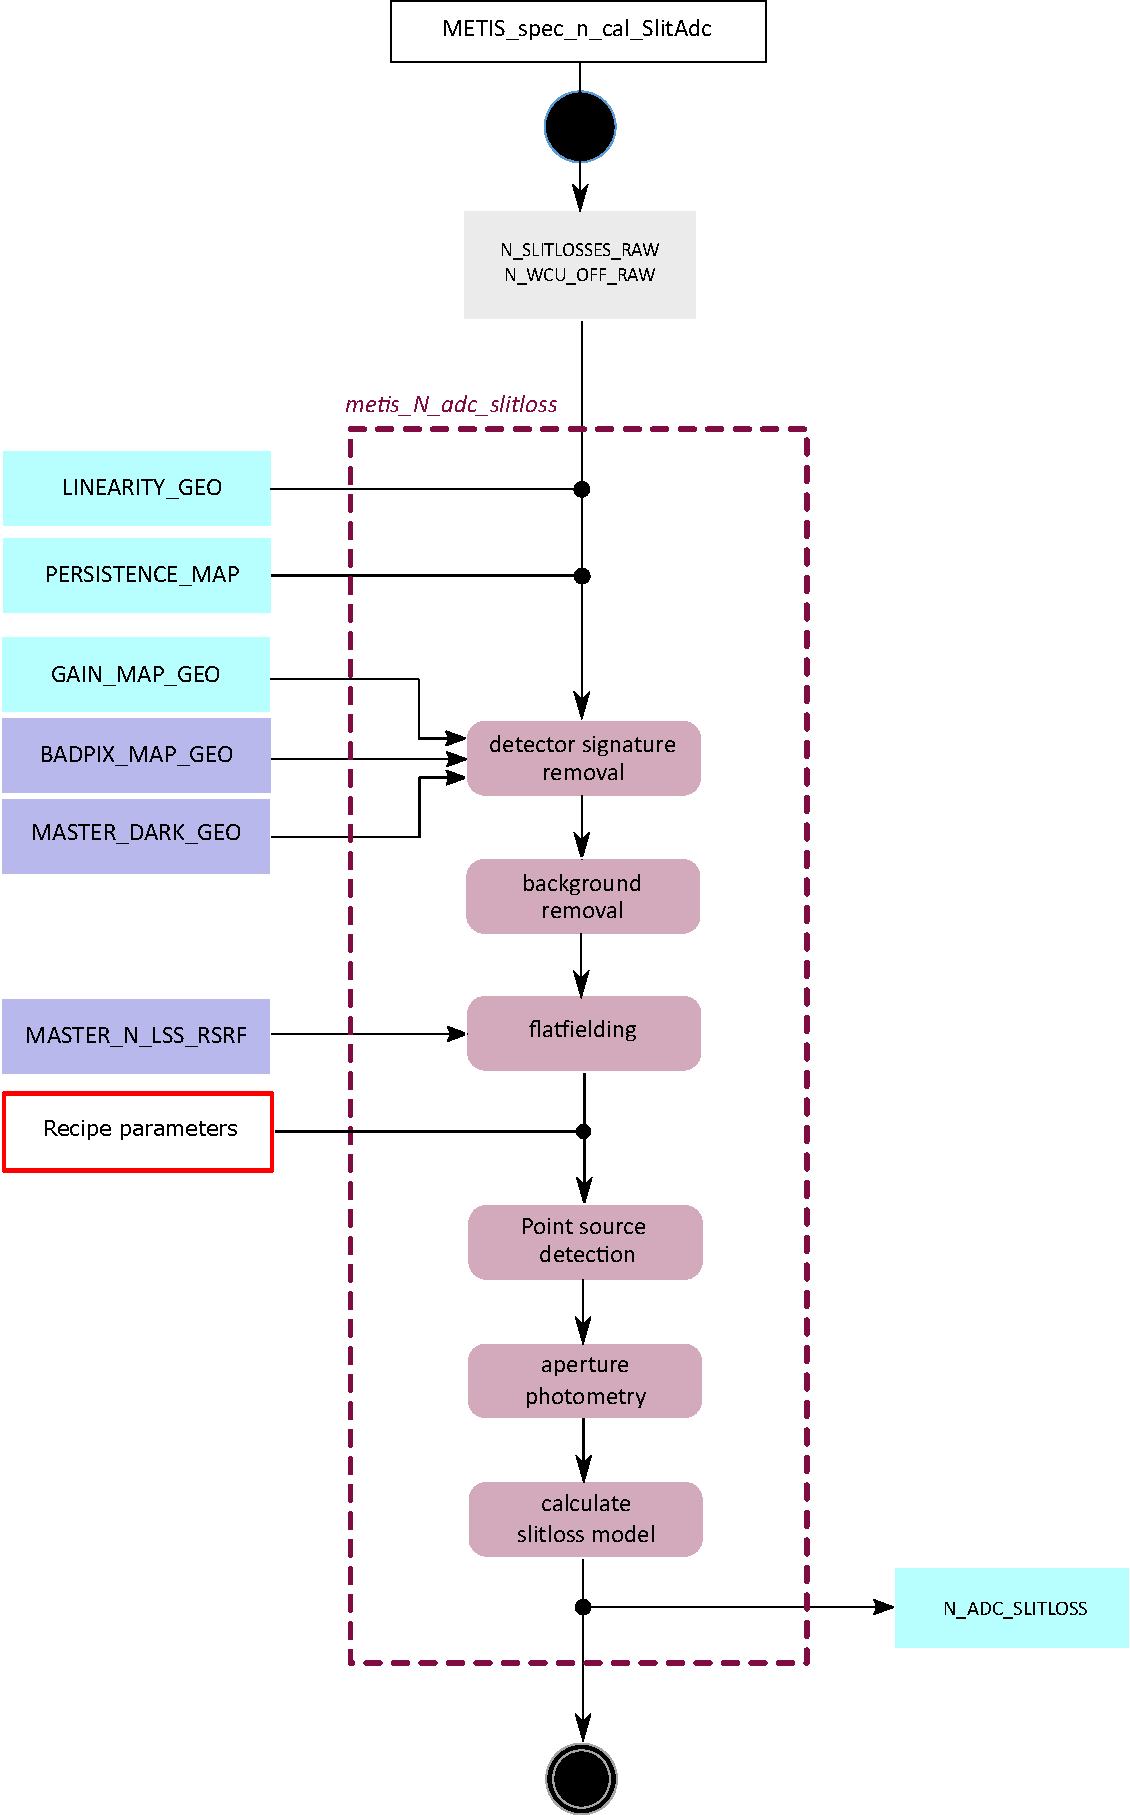
\includegraphics[width=0.5\textheight]{figures/metis_n_lss_adc_slitloss_v0.83.pdf}
  \caption[Recipe: \REC{metis_n_adc_slitloss}]{\REC{metis_n_adc_slitloss} --
    Recipe workflow to determine the \ac{ADC} induced slit losses.}
  \label{Fig:rec_n_adc_slitloss}
\end{figure}

\begin{recipedef}\label{rec:metisnadcmslitloss}\label{rec:metis_n_adc_slitloss}
Name:		& \hyperref[rec:metis_n_adc_slitloss]{\REC{metis_n_adc_slitloss}} \\
Purpose:	& Determination of the \ac{ADC} induced slit losses \\
Type:		& Calibration\\
Requirements: & METIS-6074, METIS-2757, METIS-9099, METIS-9150 \\
Input data:     & \hyperref[dataitem:n_slitlosses_raw]{\RAW{N_SLITLOSSES_RAW}} \\
                & \hyperref[dataitem:n_wcu_off_raw]{\RAW{N_WCU_OFF_RAW}} \\
                & \hyperref[dataitem:persistence_map]{\EXTCALIB{PERSISTENCE_MAP}}  \\
                & \hyperref[dataitem:linearity_geo]{\STATCALIB{LINEARITY_GEO}}  \\
                & \hyperref[dataitem:gain_map_geo]{\PROD{GAIN_MAP_GEO}}  \\
                & \hyperref[dataitem:badpix_map_geo]{\PROD{BADPIX_MAP_GEO}}  \\
                & \hyperref[dataitem:master_dark_geo]{\PROD{MASTER_DARK_GEO}}  \\
                & \hyperref[dataitem:master_img_flat_lamp_n]{\PROD{MASTER_IMG_FLAT_LAMP_N}}  \\
Parameters: 	& exposure time, offset positions\\
Algorithm:      & remove detector signature\\
                & remove dark\\
                & apply flatfield\\
                & detect reference source from \ac{WCU} via centroid peak detection\\
                & apply aperture photometry\\
                & calculate (simple) slitloss model (details to be defined)\\
Output data:	& \hyperref[dataitem:n_adc_slitloss]{\STATCALIB{N_ADC_SLITLOSS}} (Slit loss model as function of the wavelength and object position across the slit) \\
Expected accuracies: & 3\% (cf. \cite{METIS_calerrbudget})\\\\
%QC1 parameters: & \QC{TBD}: TBD\\
\end{recipedef}


%%% Local Variables:
%%% mode: latex
%%% TeX-master: "METIS_DRLD"
%%% End:
